%%%%%%%%%%%%%%%%%%%%%%%%%%%%%%%%%%%%%%%%%%%%%%%%%%%%%%%%%%%%%%%%%%%%%%%%%%%%%
%
%  System        : 
%  Module        : 
%  Object Name   : $RCSfile$
%  Revision      : $Revision$
%  Date          : $Date$
%  Author        : $Author$
%  Created By    : Robert Heller
%  Created       : Sat Apr 15 10:32:29 2023
%  Last Modified : <230415.1032>
%
%  Description 
%
%  Notes
%
%  History
% 
%%%%%%%%%%%%%%%%%%%%%%%%%%%%%%%%%%%%%%%%%%%%%%%%%%%%%%%%%%%%%%%%%%%%%%%%%%%%%
%
%    Copyright (C) 2023  Robert Heller D/B/A Deepwoods Software
%			51 Locke Hill Road
%			Wendell, MA 01379-9728
%
%    This program is free software; you can redistribute it and/or modify
%    it under the terms of the GNU General Public License as published by
%    the Free Software Foundation; either version 2 of the License, or
%    (at your option) any later version.
%
%    This program is distributed in the hope that it will be useful,
%    but WITHOUT ANY WARRANTY; without even the implied warranty of
%    MERCHANTABILITY or FITNESS FOR A PARTICULAR PURPOSE.  See the
%    GNU General Public License for more details.
%
%    You should have received a copy of the GNU General Public License
%    along with this program; if not, write to the Free Software
%    Foundation, Inc., 675 Mass Ave, Cambridge, MA 02139, USA.
%
% 
%
%%%%%%%%%%%%%%%%%%%%%%%%%%%%%%%%%%%%%%%%%%%%%%%%%%%%%%%%%%%%%%%%%%%%%%%%%%%%%

\section{General Wiring Notes}

\subsection{Main board}
\begin{figure}[hbpt]\begin{centering}%
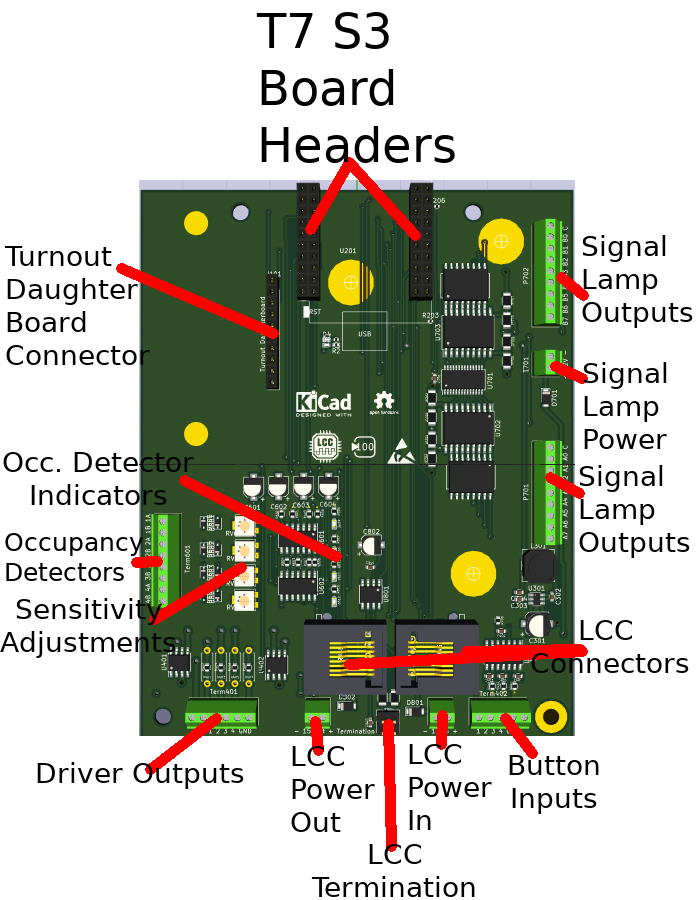
\includegraphics[width=5in]{ESP32-T7S3-MultiFunctionUniversalTurnout-Annotated.png}
\caption{ESP32 T7S3 MultiFunctionUniversalTurnout board, annotated}
\end{centering}\end{figure}

There are various terminal blocks, connectors, and jumper blocks on this
board.  

On the left side is a 10 position socket header for the turnout daughter board
and an 8 position terminal block for the four CT coil occupancy detectors,
Along the bottom is the 6 position terminal block for the driver outputs, then
come the terminal block to extracting power from the LCC bus. Then there is
the termination jumper block for the LCC bus. Then there is terminal block for
injecting power into the LCC bus. Above the LCC power terminal blocks is a
pair of RJ45 connectors. These are for connecting the board to the LCC bus.
These connectors are wired in parallel. On the right side of the board are two
9 position terminal blocks for the signal lamp LEDs. Finally, between the
terminal blocks for the signal lamp LEDs is a two position terminal block to
(optionally) provide power for the signal lamp LEDs.

\subsubsection{Turnout Daughter board connector}

Starting on the upper left, there is a 10 position socket header for the 
turnout daughter board.  The socket mates with the 10 position pin array on 
the underside of the Turnout Daughter board.  The Turnout Daughter boards' 
terminal blocks are described below in Sections~\ref{sect:SM-Daughter}, 
\ref{sect:TS-Daughter}, \ref{sect:SC-Daughter}, and \ref{sect:TC-Daughter}.

\clearpage
\subsubsection{Occupancy Detectors}
\begin{figure}[hbpt]\begin{centering}%
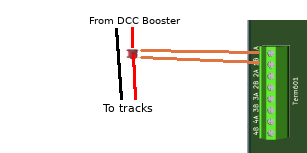
\includegraphics[height=1.5in]{OccupancyDetector-Wiring.png}
\caption{Occupancy Detector Wiring}
\end{centering}\end{figure} 

Then on the lower left side is an 8 position terminal block for the four CT 
coil occupancy detectors.  Each adjacent pair of terminals is for one twisted 
pair cable to one CT coil for one feeder wire for one block. There is a 
sensitivity adjustment trimmer and an indicator LED for each detector.

\subsubsection{Driver Outputs}

There is a 6 position terminal block for the four driver outputs. There are
1500 Ohm load resistors on board, which are suitable for driving LEDs with a
12V supply. There are places for adding through hole load resistors to allow
for increased load current. The driver outputs require an external power
source, typically 12V. The driver chips are totem pole (push-pull), so can
drive both high side and low side, up to 1.5 Amps.

\subsubsection{LCC Power}

Power can be optionally injected into the LCC bus or extracted from the LCC 
bus. Power can be injected to into the LCC bus to power this and other boards. 
Power can also be extracted to power local devices.

\subsubsection{LCC Network Connectors}

There are two RJ45 connectors for the LCC Network. Connect a CAT5 or CAT6
(Ethernet) cable of at least 1 foot in length to the next and previous node in
the network. If this is the last node, only one connector is used and
termination jumpers should be installed. See Section~\ref{sect:termination}.

\subsubsection{Button (or switch) Inputs}

There is a 5 position terminal block for button (or switch) inputs.  These are 
Schmitt-trigger inputs and are referenced to ground (supplied on the fifth 
position of the terminal block).

\subsubsection{PWM Signal Lamp drivers}

There are two 9 position terminal blocks for the sixteen PWM Signal Lamp 
outputs (two banks of 8) and there is a two position terminal blocks to 
provide (optional) external power for the signal lamps.  These terminal blocks 
are on the right side of the board.  The boards can be build to be either for 
common anode or common cathode.

\clearpage
\subsubsection{LCC Termination}
\label{sect:termination}
\begin{figure}[hbpt]\begin{centering}%
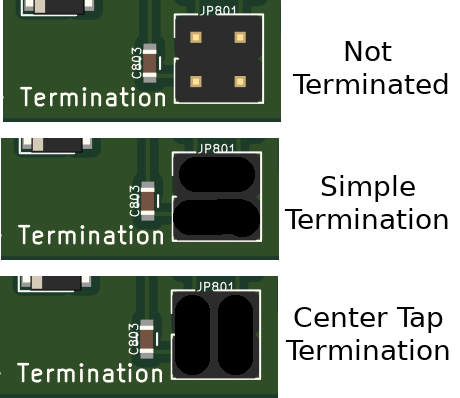
\includegraphics{TerminationJumpers.png}
\caption{Termination Options}
\label{fig:termination}
\end{centering}\end{figure}

There are three options for termination: none, simple, and center tap, as 
shown in Figure~\ref{fig:termination}.


\subsection{Stall Motor Turnout daughter board}
\label{sect:SM-Daughter}
\begin{figure}[hbpt]\begin{centering}%
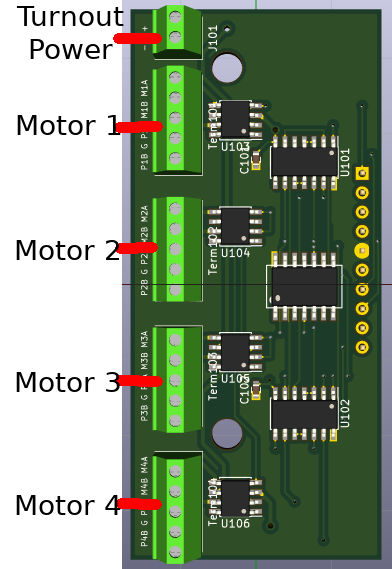
\includegraphics[height=2.5in]{SM-DaughterBoard-Annotated.png}
\caption{Stall Motor Turnout daughter board, annotated}
\end{centering}\end{figure}
\begin{figure}[hbpt]\begin{centering}%
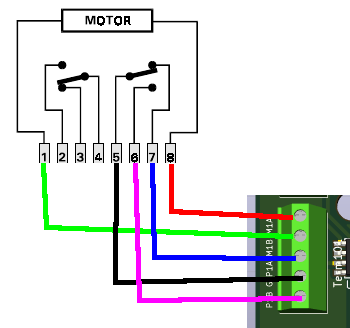
\includegraphics[height=1.5in]{SM-DaughterBoard-TortoiseWiring.png}
\caption{Stall Motor Turnout daughter board, wired to a Tortoise.}
\end{centering}\end{figure}


The Stall Motor Turnout daughter board can drive Circuitron Tortoise and
similar slow motion, stall motor switch machines. There is a 2 position
terminal block for a 12-15 volt supply to drive the stall motors and four 5
position terminal blocks, one for each motor. Each 5 position terminal block
has motor A and B connection for the motors and a point A and B and a ground
(G) connection for the point sense. The motor A and B connections go to the
Tortoises 1 and 8 pins, and the other three can be connected to one of the
poles of the internal switch contacts to report point sense -- the G to the
common.

\subsection{Servo Turnout daughter board}
\label{sect:TS-Daughter}
\begin{figure}[hbpt]\begin{centering}%
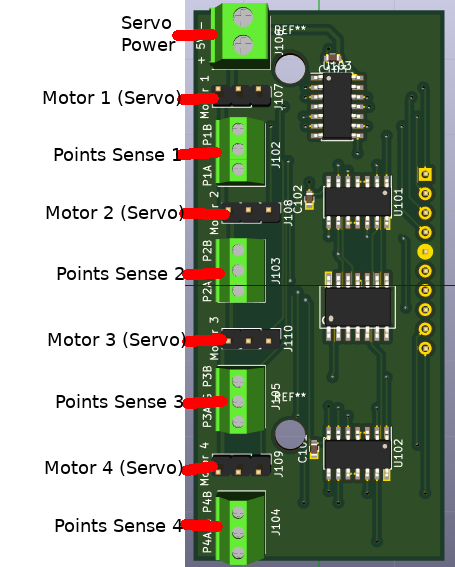
\includegraphics[height=2.5in]{TS-DaughterBoard-Annotated.png}
\caption{Servo Turnout daughter board, annotated}
\end{centering}\end{figure}

The Servo Turnout daughter board can drive standard 5V servos. There a 2
position terminal block for a 5 volt power supply to drive the servos, four
3-pin headers for standard servo connectors, along with four 3 position
terminal blocks for point sense.

\subsection{Single Coil Turnout daughter board}
\label{sect:SC-Daughter}
\begin{figure}[hbpt]\begin{centering}%
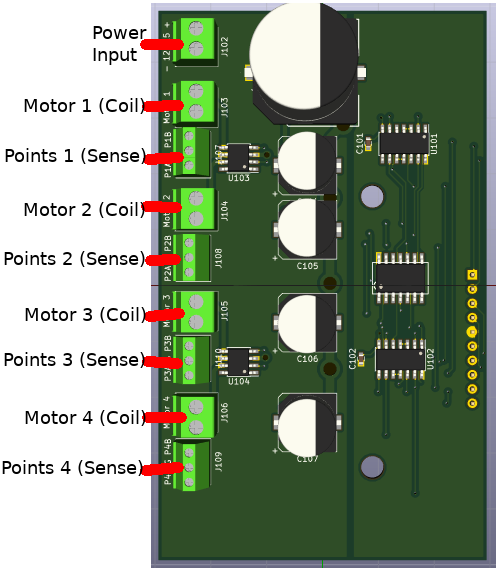
\includegraphics[height=2.5in]{SC-DaughterBoard-Annotated.png}
\caption{Single Coil Turnout daughter board, annotated}
\end{centering}\end{figure}

The Single Coil Turnout daughter board can drive single coil snap action
turnouts, typically Kato turnout motors. This a capacitive discharge type
driver circuit. There is a 2 position terminal block for a 12-15 volt power
supply to charge the capacitors.  There is a larger 2 position terminal block 
for each coil, along with a smaller 3 position terminal block point sense for 
each of four turnouts.

\subsection{Twin Coil Turnout daughter board}
\label{sect:TC-Daughter}
\begin{figure}[hbpt]\begin{centering}%
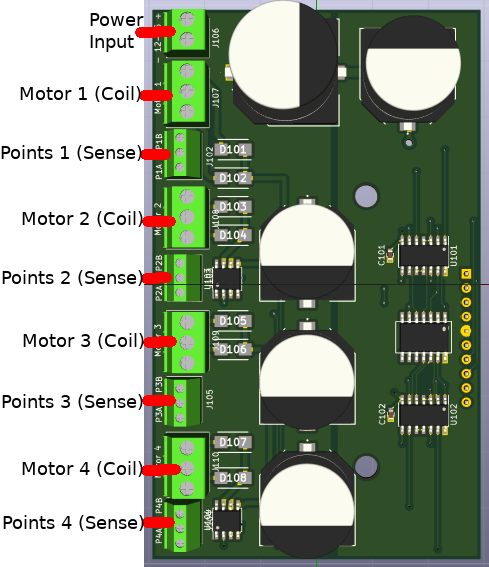
\includegraphics[height=2.5in]{TC-DaughterBoard-Annotated.png}
\caption{Twin Coil Turnout daughter board, annotated}
\end{centering}\end{figure}                                                    
 
The Twin Coil Turnout daughter board can drive twin coil snap action turnouts,
such as Atlas or Peco switch machines. This a capacitive discharge type driver
circuit. There is a 2 position terminal block for a 12-15 volt power supply to
charge the capacitors. There is a larger 3 position terminal block for each
pair of coils, along with a smaller 3 position terminal block point sense for
each of four turnouts.

\clearpage
